\documentclass[12pt,a4paper,twoside]{article}
\usepackage[utf8]{inputenc}
\usepackage{amsmath}
\usepackage{lmodern}
\usepackage{textcomp}
\usepackage{amsfonts}
\usepackage{amssymb}
\usepackage{graphicx}
\usepackage[left=2cm,right=2cm,top=2cm,bottom=2cm]{geometry}
\author{Cabello Lopez Marco Antonio\\
Actividad 6\\
Departamento de Fisica\\
Universidad de Sonora}
\date{Hermosillo, Sonora a Jueves 30 de Noviembre del 2017}
% used in maketitle                                                             
\title{\textbf{Sistema Sol-Tierra-Luna}}
\begin{document}
\maketitle
\section{Planteamiento del problema}
En esta actividad se pide calcular algunos parametros del movimiento de traslacion de un sitema que contiene a  nuestro planeta, la luna y el sol apoyados con Fortran.\\
Apoyandonos con las notas del movimiento circular uniforme y con las funciones intrinsecas que son necesarias para poder realizar el proceso a traves de las subrutinas del programa.

\begin{figure}[h!]
  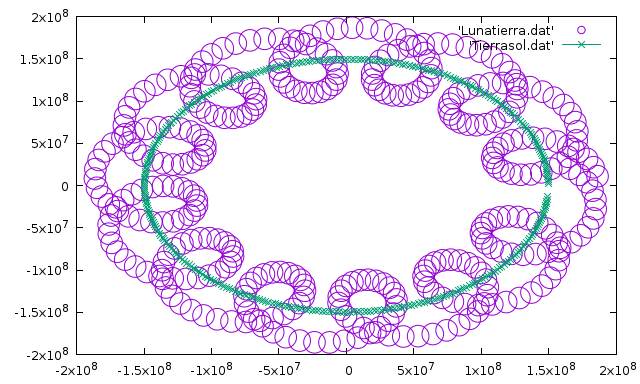
\includegraphics[width=\linewidth]{MoonEarthSun.png}
  \caption{Sistema Sol-Tierra-Luna}
  \label{fig:Grafica}
\end{figure}
\clearpage


\maketitle
\section{Movimiento de Traslación de la Tierra y La Luna}
La traslación es el movimiento en el cual la Tierra orbita alrededor del Sol. La distancia promedio entre estos cuerpos es de 149,600,000 kilometros, tomando por lo tanto un tiempo total de 365.256 dias en completar su orbita el planeta Tierra.\\
La distancia media entre la Tierra y la Luna es 384.400 kilometros, la distancia real varia a lo largo de la orbita de la Luna. La Luna tarda en dar una vuelta alrededor de la Tierra 27.3217  dias en completar una vuelta a la Tierra.\\

\clearpage
\section{Codigo del programa}
\begin{verbatim}
FUNCTION solx(angsol) RESULT (x)
	double precision, intent(IN) :: angsol
	double precision 	     :: x
        double precision, parameter :: rsolar = 1.496d8
	 x = rsolar * dcos(angsol)
END FUNCTION solx

FUNCTION soly(angsol) RESULT (y)
	double precision, intent(IN) :: angsol
	double precision 	     :: y
	double precision, parameter :: rsolar = 1.496d8
	 y = rsolar * dsin(angsol)
END FUNCTION soly

SUBROUTINE moonearth(rsolar, rlunar, posx, posy, anglun, angsol)
   double precision, intent (IN) :: rsolar, anglun, angsol
   double precision, intent (OUT) :: posx, posy
   double precision :: rlunar
   rlunar = rsolar / 4.0d0
   posx = (rsolar * dcos(angsol)) +(rlunar * dcos(anglun))
   posy = (rsolar * dsin(angsol)) +(rlunar * dsin(anglun))
 
END SUBROUTINE moonearth 


PROGRAM moon
	IMPLICIT NONE
	integer :: i
	double precision :: g, dia, rsolar, rlunar, posx, posy, anglun
	double precision :: rad, velocidadlun, velocidadsol, solx, soly, angsol
	double precision, parameter :: pi=3.1416d0, mes = 27.3217d0, year = 365.26d0
	double precision, dimension(360) :: totalx,totaly
	double precision, dimension(360) :: x, y
  rsolar = 1.496d8
  rad = pi / 180.0d0
  dia = 365.26d0/(360.0d0*rad) 
  velocidadlun = 2.0d0 * (pi / mes) !Calcula el trayecto diariamente la luna en radianes
  velocidadsol = 2.0d0 * (pi / year)  
  
OPEN (1, FILE = 'MoonEarth.dat', STATUS = 'unknown')
OPEN (2, FILE = 'EarthSun.dat', STATUS = 'unknown')
 DO i=1, 360, 1
 g = dble(i)
 angsol = g * velocidadsol
 anglun = g * velocidadlun  !Obtiene la posicion actual en radianes
 x(i) = solx(angsol)
 y(i) = soly(angsol) 
 CALL moonearth(rsolar, rlunar, posx, posy, anglun, angsol)  !Calcula la posicion de la luna respecto a la tierra y el sol
 totalx(i) = posx
 totaly(i) = posy
 WRITE (1,*) totalx(i), totaly(i)
 WRITE (1,*) ' '
 WRITE (2,*) x(i), y(i)
 WRITE (2,*) ' '
 
 END DO
 CLOSE (1)
 CLOSE (2)
END PROGRAM moon
\end{verbatim}




\end{document}